% ************ Chapter 2 ************
%\renewcommand{\chaptername}{Chapter}
\chapter{Estado da Arte}
\label{cap:2}
\emph{Este capitulo apresenta as alternativas mais relevantes para a descentralização da web}

%\section{Contextualização}
Assistimos hoje em dia a problemas sérios e crescentes relativos a manipulação de informação, consequentes de um paradigma de web que foi explorado ao limite, por forma a criar modelos de negócio obscuros e com pouca transparência na recolha e utilização dos dados de utilizadores.

O modelo actual é um monstro gigante, onde a informação se encontra replicada infinitamente, e a camada de persistência de dados nas diferentes arquiteturas é provavelmente aquela que mais destaque tem para todas as estruturas organizacionais. Isto torna-se um problema, quando não existe respeito pelos utilizadores e a manipulação dos dados passa a ser o "core business".

Um modelo de descentralização da web, vem sendo discutido desde tempos atrás, com várias abordagens possíveis, mas sempre com a garantia de que a informação será sempre propriedade do utilizador. Neste contexto um modelo só pode emergir a partir de uma adoção massiva, que por sua vez requer um conjunto de ferramentas capazes de sustentar este processo de forma eficaz e suficientemente escalável.

\section{Modelos Descentralizados}
Nesta secção são apresentadas diferentes alternativas que podem servir de base para um novo paradigma de web descentralizada. Para tal devem ser soluções robustas e que ofereçam ferramentas auxiliares para o desenvolvimento e posterior integração de novas aplicações.

\subsection{Solid}
A arquitetura implícita para o desenvolvimento de aplicações baseadas em Solid permite que os utilizadores escolham um POD à sua escolha (próprio ou recorrendo a um servidor de POD) para conceder às aplicações autorização para armazenar ou ler informação a partir do mesmo. Por si só, este facto permite que os utilizadores escapem dos tradicionais "silos de dados". Além disto, esses PODs podem oferecer diferentes granularidades de privacidade, confiabilidade, disponibilidade, proteção legal e reutilização de dados.\cite{solid_official}

O Solid implementa atualmente dois mecanismos de autenticação alternativos, o WebID-TLS e o WebID-OIDC. \cite{solid_spec}

O WebId-TLS utiliza identificadores exclusivos com a ajuda de certificados criptográficos para provar a identidade do utilizador. \cite{solid_webid-tls:}

O WebId-OIDC é baseado nos protocolos OAuth2/ OpenID Connect, adaptado para casos de uso descentralizados. \cite{solid_webid_oidc}

Além disso, existem outros métodos de autenticação atualmente em fase de investigação.

Relativamente à persistência de informação, o Solid recorre aos PODs (Personal online datastores) para conseguir alcançar persistência descentralizada, que atua como a camada de backend para as aplicações. Os Pods disponibilizam interfaces Rest baseadas em Linked Data Platform (LDP), uma recomendação da comunidade W3C, assim como um mecanismo baseado em queries SPARQL.\cite{solid_spec}

\begin{figure}[h]
    \begin{center}
    % Requires \usepackage{graphicx}
    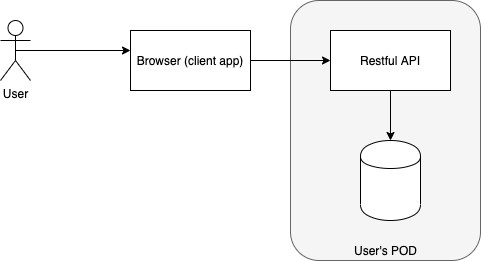
\includegraphics[width=1\textwidth]{figures/estado_arte-Solid.png}
    \caption{Representação SOLID}
    \end{center}
\end{figure}

\subsection{Blockstack}
Blockstack é um projeto open-source que pretende construir uma rede de computação descentralizada assente na camada de transporte da Internet e protocolos de comunicação subjacentes. Para atingir este estatuto, está assente nas seguintes camadas:
\begin{itemize}
	\item Stacks Blockchain - Permite aos utilizadores controlar e register ativos digitais, como usernames e passwords ou executar contratos inteligentes.\cite{blockstack_white_paper}
	\item Gaia - Armazenamento descentralizado
	\item Blockstack Authentication - Protocolo que permite autenticação descentralizada.\cite{blockstack_white_paper}
	\item Libraries and SDKs - Ferramentas para facilitar o desenvolvimento de aplicações baseadas em Blockstack. \cite{blockstack_white_paper}
\end{itemize}

Um dos conceitos chave da arquitetura desta plataforma é o sistema de ficheiros descentralizado chamado Gaia Hub, que permite aos utilizadores escolher e providenciar o seu repositório de informação.

Assim como o Solid, Blockstack tem também um um sistema de armazenamento descentralizado baseado em Gaia Hubs, repositórios de informação privados que podem também ser partilhados entre a comunidade ou podem apenas ser propriedade de cada utilizador. 

Estes repositórios disponibilizam uma interface de aplicação RESTful, permitindo que as aplicações adicionem informação através de pedidos POST, sendo que cada pedido deve ser acompanhado por um token autenticação assinado e validado pelo repositório. Cada aplicação tem uma chave privada que confere acesso a uma partição especifica do repositório impedindo que, ao contrário do Solid, possa haver partilha de informação entre as diferentes aplicações.\cite{blockstack_white_paper}

Em termos de autenticação, consegue providenciar autenticação descentralizada através do mecanismo de autenticação por chave pública criptográfica. A partir do login, a aplicação recebe três peças essenciais de informação: o nome de utilizador, uma chave privada específica de aplicação e a localização do repositório para armazenar informação.\cite{blockstack_white_paper}

\begin{figure}[h]
    \begin{center}
    % Requires \usepackage{graphicx}
    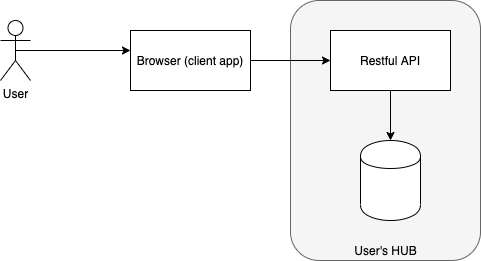
\includegraphics[width=1\textwidth]{figures/estado_arte-Blockstack.png}
    \caption{Representação Blockstack}
    \end{center}
\end{figure}

\subsection{Diaspora}
Diaspora é um projeto com uma visão um pouco mais reduzida que as restantes alternativas, na medida em que foca-se apenas em apresentar um protótipo daquilo que poderia ser uma rede social descentralizada. Este projeto assenta em servidores de informação independentes, que o utilizador pode escolher ou até mesmo configurar o seu. \cite{diaspora_wiki}

O conceito principal desta rede é o POD (assim como no Solid), a sua arquitetura é relativamente intuitiva, tendo as aplicações a interagir com as instâncias servidoras distribuídas pelo mundo. Estes servidores são mantidos em sincronização utilizando a tecnologia WebSub. \cite{diaspora_wiki}

Relativamente a autenticação, não é adotado nenhum mecanismo fora do comum, sendo apenas o método comum username/password.

\begin{figure}[h]
    \begin{center}
    % Requires \usepackage{graphicx}
    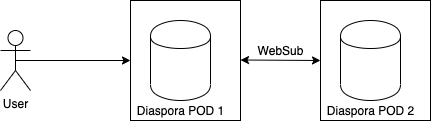
\includegraphics[width=1\textwidth]{figures/estado_arte-Diaspora.png}
    \caption{Representação Diaspora}
    \end{center}
\end{figure}

\subsection{Elastos}
Elastos incide no desenvolvimento de um novo paradigma de web potenciado por tecnologia blockchain. O foco principal incide não só na proteção dos dados, mas também na defesa dos direitos de autor. A plataforma é constituída por quatro componentes:\cite{elastos_white_paper}
\begin{itemize}
	\item Elastos Blockchain
	\item Elastos Runtime
	\item Elastos Carrier
	\item Elastos SDK
\end{itemize}

O conceito baseia-se num sistema operativo relativamente leve que armazena a informação e previne que as aplicações e serviços tenham ligação à Internet. Toda a informação tem identificadores providenciados por Blockchain (pode ser Bitcoin ou uma rede de Blockchain alternativa), sendo estes IDs verificados antes de os ativos digitais serem transmitidos entre as diferentes máquinas virtuais, utilizando comunicação "peer to peer" providenciada pela camada Elastos Carrier.\cite{elastos_developer}

O sistema Elastos dispõe de um componente de armazenamento descentralizado, i.e. Elastos Hive. Recorre a um sistema de arquivos interplanetário como base. Oferece uma interface de aplicação para aceder à informação que será dispersa pelas diferentes regiões do planeta, garantindo assim fiabilidade às aplicações.\cite{elastos_white_paper}

Relativamente à autenticação, esta plataforma introduz um ID descentralizado (DID), construído na rede Blockchain e providencia IDs confiáveis para tudo e para todos. 

O ID pode ser utilizado para efeitos de rastreamento, autenticação e estabelecimento de ligações seguras. De forma simplificada, a camada Elastos Carrier é a combinação entre DID e a comunicação P2P, assegurando assim que a informação é transmitida em segurança após a autenticação e a autorização serem devidamente validadas.\cite{elastos_white_paper}

\begin{figure}[h]
    \begin{center}
    % Requires \usepackage{graphicx}
    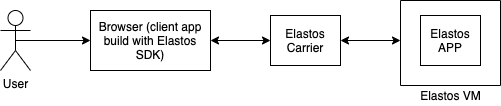
\includegraphics[width=1\textwidth]{figures/estado_arte-Elastos.png}
    \caption{Representação Elastos}
    \end{center}
\end{figure}
